%!TEX encoding = UTF-8 Unicode
%!TEX root = ./../main.tex
%!TEX TS-program = xelatex

\chapter[OBP App.]{Observation Pack Approssimato} % chapter 6 title
\label{cap:sei}
L'obiettivo di questo lavoro è indagare la capacità di apprendere linguaggi regolari in uno scenario di \textit{Active Learning}, nel caso in cui non si disponga di un \textit{Oracolo} capace di rispondere nativamente nè ad \ac{EQ} nè a \ac{MQ}\footnote{L'\textit{Oracolo} è approssimato tramite un classificatore che è in grado per sua natura di rispondere a una \textit{membership query}. Qui si intende che non è in grado di rispondere a una \ac{MQ} tramite il \ac{DFA} target perchè quest ultimo è considerato incognito nel processo inferenziale}.  
In letteratura esistono diversi algoritmi utilizzati per  l'appredimento di linguaggi regolari. 
L' approssimazione dell' \textit{Oracolo} è  indipendente dallo specifico algoritmo d'\ac{IIR}, tuttavia per renderlo concreto l'attenzione è stata focalizzata sull'\ac{ObP}.
 Si è scelto di utilizzare \ac{SVM} come classificatore atto a modellare un \textit{Oracolo}, classificatore costruito a partire da alcuni esempi positivi e negativi del linguaggio da apprendere. Sarebbe opportuno preventivamente leggere le Appendici \ref{cap:cinque}  e \ref{app:tre} dato che i concetti e le tecniche lì descritte sono propedeudiche all'algoritmo qui delineato.\\
 Data la natura non esatta dell'algoritmo ivi realizzato questo viene indicato come \ac{ObPA}.\\
  Corredata a questa tesi vi è anche l'implementazione dell' \ac{ObP} in C++11 , codice che è stato integrato in  Gi-learning \cite{Cot16} una libreria preesistente. Nelle applicazioni reali tuttavia è altamente improbabile la disponibilità di un \textit{Oracolo} in grado di rispondere a delle \ac{EQ} da cui l'esigenza di un \textit{Oracolo approssimato} e dell'\ac{ObPA} la cui relativa implementazione oggetto di tesi è stata parimenti integrata in  Gi-learning \cite{Cot16}.

\section{Precedenti lavori in letteratura}
Assumere che il \textit{teacher} sia in possesso del linguaggio target \ac{L} è uno scenario poco plausibile essendo esso stesso l'oggetto dell'inferenza.
Quindi l'obiettivo delineato in questa tesi è indagare il comportamento di un algoritmo di \textit{active learning} per inferire il \ac{DFA} A tale che $L(A) =\ac{L}$ tramite un oracolo approssimato realizzato con un classificatore statistico e tale intento si discosta dai lavori preesistenti in letteratura. In realtà una prima versione di un algoritmo di \textit{active learning} che realizza un Oracolo approssimato è già presente in Angluin \cite{Angluin87} in cui si approssima un \ac{EQ} tramite un certo numero di \ac{MQ} nella sua versione di L* approssimato. Più di recente, nella stessa direzione è andata la competizione Zulu \cite{Zulu10}: il vincitore della competizione \cite{Howar12} definisce il nuovo tipo di query: l'  \textit{Identity Query}
\begin{definizione*}[Identity Query] Testa se due prefissi $u,u'$ sono nella stessa classe di equivalenza del target A cioè se $u \not\simeq_{\lambda^{A}} \! u'$. In caso $u \not\simeq_{\lambda^{A}} \! u'$ ritorna un suffisso $v$ per il quale $\lambda^{A}(uv) \neq \lambda^{A}(u'v)$. Altrimenti ritorna il successo. 
\end{definizione*}
e dimostra che i linguaggi regolari possono essere inferiti con un numero polinomiale di \ac{MQ} ed \textit{Identity Query}.       
Le \textit{Identity Query} non sono meno realistiche delle \ac{EQ} ma tramite esse è possibile definire un framework che consente di approssimare in maniera relativamente facile ed efficiente un'\textit{Identity Query} tramite \ac{MQ}.  Anche gli altri algoritmi in letteratura sono focalizzati sulla ricerca di algoritmi che in maniera efficiente riescono ad approssimare le \ac{EQ} tramite \ac{MQ}.  In questa sede si assume invece l'impossibilità di rispondere nativamente anche alle \ac{MQ} oltre che alle \ac{EQ}, cioè  anche l'esito delle \ac{MQ} non è noto ed andrà approssimato.

Per quanto concerne la selezione del classificatore statistico per approssimare l'Oracolo la scelta è ricaduta su \ac{SVM} perchè costituiscono un modello molto potente. Inoltre sono poche le applicazioni delle \ac{SVM} per l'apprendimento di linguaggi regolari come in \cite{Clark11}\cite{Clark06}  in cui si riesce a definire un kernel string utile per l'apprendimento dei linguaggi planari\footnote{I linguaggi planari sono una classe di linguaggi che attraversano la tassonomia di Chomsky nel senso che apprendono solo in maniera parziale i linguaggi finiti,regolari,context-free,context-sensitive ecc. senza saturare nessuno di essi}  oppure in \cite{Kontorovich09} dove si delinea un lavoro teorico sui linguaggi regolari e si propone un kernel string senza concretizzarlo specificamente per l'apprendimento di linguaggi regolari nell'accezione dell'\textit{active learning}. Altri tipi di classificatori come ad esempio le \textit{Recurrent Neural Network} si sono rilevate particolarmente adatte allo scopo di modellare un \ac{DFA} ma come si evince da \cite{Forcada02}, che definisce una panoramica su di esse a riguardo dell'impiego in  \ac{GI}, sono state già ampiamente dibattute in letteratura.

\section{Introduzione ObPA}
Una preliminare osservazione per evitare la creazione di ambiguità nel prosieguo consiste nel rimarcare che il codice prodotto è costituito da una duplice versione. Vi è infatti il codice riguardante la fase di \textit{debug} riferito d'ora in avanti come \textit{ideal version} e quello pronto per l'utilizzo reale riferito d'ora in avanti come \textit{release version}
%\footnote{In realtà esiste un unica versione del codice ma si passa da una versione all'altra attivando o disattivando il flag in compilazione DEBUG$\_$EVALUATION (se è definito si sta optando per la \textit{ideal version})}.
  Con l'intento di spiegare le differenze principali tra le due versioni e contemporaneamente introdurre l'\ac{ObPA} vengono forniti gli pseudocodici \ref{alg:obpad} e \ref{alg:obpar} di alto livello:

\begin{algorithm}
\caption{OBPA \textit{ideal version}}\label{alg:obpad}
\begin{algorithmic}[1]
\Statex
\Input il \ac{DFA} target $A$,l' alfabeto $\Sigma$ 
\Output il \ac{DFA} inferito $Ob\_DFA$
\State $samples \gets A.random\_walk(750,750)$
\State $training\_set \gets pull\_out(samples,500)$
\State $test\_set \gets pull\_out(samples,1000)$
\State $appr\_oracle \gets \textbf{new}\:\: appr\_oracle(|\Sigma|,\Sigma,training\_set,test\_set)$
 \LineComment{Sul training\_set si addestra SVM e con il  \textit{test\_set} si fa model evaluation}
\State $Ob\_DFA \gets OBSERVATION\_PACK(appr\_oracle).run()$
\State $statistical\_measure \gets compare(Ob\_DFA , A)$
 \State \textbf{return} $Ob\_DFA$
     
\end{algorithmic}
\end{algorithm}




\begin{algorithm}
\caption{OBPA \textit{release version}}\label{alg:obpar}
\begin{algorithmic}[1]
\Statex
\Input l' alfabeto $\Sigma$
\Output il \ac{DFA} inferito $Ob\_DFA$
\State $training\_set \gets read\_file(path\_file)$ \Comment{Nel file samples disponibili all'utente}
\State $appr\_oracle \gets \textbf{new}\:\: appr\_oracle(|\Sigma|,\Sigma,training\_set)$
 \LineComment{Sul training\_set si addestra SVM e non si effettua  model evaluation}
\State $Ob\_DFA \gets OBSERVATION\_PACK(appr\_oracle).run()$
 \State \textbf{return} $Ob\_DFA$
     
\end{algorithmic}
\end{algorithm}

La differenza principale tra le due versioni è che nella \textit{ideal version} si è in possesso del \ac{DFA} target e nella \textit{release version} non si possiede in alcun modo questa conoscenza.  Si generano 1500 campioni bilanciati campioni con un particolare algoritmo ,\textbf{random walk}.  Dai campioni iniziali si estraggono il \textit{training set} di 500 elementi e il \textit{test set} composto dai rimanenti 1000. Si crea un oracolo approssimato che provvede internamente a costruire un classificatore a partire dal \textit{training set} e usa il \textit{test set} per valutare il classificatore scelto. Si invoca l'\ac{ObP} passandogli l'Oracolo approssimato; \ac{ObP} funziona in maniera classica come descritto nel capitolo \ref{cap:quattro} ma al momento di invocare i metodi per effettuare le \ac{MQ} ed \ac{EQ} saranno chiamati i metodi dell'Oracolo approssimato  che saranno realizzati mediante il classificatore precedentemente costruito. Viene inferito un \ac{DFA} che viene confrontato con il \ac{DFA} target tramite delle misure statistiche (cfr. App. \ref{sub:measure}) .  L'algoritmo \textit{random walk} nonchè la scelta della dimensione del \textit{training set} e del \textit{test set}  e come avviene il confronto tra il target e il \ac{DFA} inferito sarà spiegato più approfonditamente nella sezione \ref{sec:gensam}.\\
Nella \textit{release version}, non essendo in possesso di un \ac{DFA} target (come accade del resto in uno scenario reale) i campioni in possesso dell'utente vengono inseriti su un file e una volta caricati nel programma costituiscono essi stessi il \textit{training set}. Come per la \textit{ideal version} si costruisce un Oracolo approssimato ma non si effettua model evaluation (non c'è un \textit{test set}) per ragioni che verranno chiarite in seguito. Alla stregua di quanto descritto per la \textit{ideal version} si inferisce un \ac{DFA} mediante l'algoritmo \ac{ObP} ma non è possibile effettuare una comparazione di quest ultimo con il \ac{DFA} target dato che è ignoto. \\
%Si puntualizza che la \textit{release version} è stata implementata generando i %campioni comunque su un \ac{DFA} target anzichè inserirli e poi leggerli da file %proprio per non doversi sobbarcare  l'onere di generare manualmente i campioni. 

\section{Costruzione del classificatore}
Come capita spesso nell'addestramento di un classificatore  sono molti gli \textit{iperparametri} da potere regolare e le possibili strade perseguibili per ricercare una soluzione soddisfacente. Per questo motivo sono state realizzate tre diverse implementazioni nominate in seguito come \ac{ObPA}1 \ac{ObPA}2 e \ac{ObPA}3. Per ognuna di esse vi è sia una \textit{ideal version} che una \textit{release version} e lo pseudocodice illustrato negli algoritmi \ref{alg:obpad} e \ref{alg:obpar} rimane valido, ma tra un'implementazione e l'altra cambiano le tecniche utilizzate per costruire il classificatore per l'oracolo approssimato a partire dal \textit{training set}.

\subsection{Libreria esterna per SVM}
Come già evidenziato in precedenza il modello prescelto è \ac{SVM} e la libreria esterna scelta è l'implementazione di Thorsten Joachims nella versione $\ac{SVM}^{light}$ (cfr. App. \ref{sec:light}). Qui si aggiungono ulteriori peculiarità riguardanti $\ac{SVM}^{light}$ in contrapposizione alla libreria GI-learning
\begin{itemize}
\item è in linguaggio C mentre la libreria GI-learning è in C++
\item è concepita come un eseguibile pronto all'uso
\item è una libreria povera  in termini di tecniche di \textit{data processing} e model selection

\end{itemize}
 Quindi è stato necessario un notevole sforzo implementativo per aggiungere alcune funzionalità di cui si parlerà a breve (k-fold-validation, codifica, scaling ecc.) e per integrare la libreria \ac{SVM} all'interno di GI-learning. Inoltre non è stato possibile utilizzare  $\ac{SVM}^{light}$ come una \textit{black-box} ma ispezionarla a basso livello per modificare alcuni aspetti e funzionalità per riadattarle agli scopi di \ac{ObPA}.\\

\subsection{ObPA1}
L'algoritmo \ac{ObPA}1 (relativamente all'addestramento del classificatore) viene presentato nell'algoritmo \ref{alg:obpa1} corrispondente a una possibile realizzazione pratica di quello che negli algoritmi \ref{alg:obpad} e \ref{alg:obpar}  è stato indicato con $appr\_oracle$.

\begin{algorithm}
\caption{OBPA1}\label{alg:obpa1}
\begin{algorithmic}[1]
\Statex
\Input a $TRS = training\_set$, a $TES = test\_set$, a $\Sigma$   
\Output $app\_oracle$
\State $encode(TRS , TES)$
\State $padding(TRS , TES)$
\State $scale(TRS , TES)$
\State $\textbf{best\_model} \gets grid\_search(TRS)$ \Comment{Si fa model selection}\label{sta:quattro}
\State $new\_best\_model \gets$ retrain $\textbf{best\_model}$ found, on whole TRS
\State $statistical\_results \gets model\_evaluation(new\_best\_model,TES)$ \label{sta:moe}
\State $\textbf{return}$ app\_oracle(new\_best\_model) 

   
\end{algorithmic}
\end{algorithm}
Nell'algoritmo \ref{alg:obpa1} è stata presentata la \textit{ideal version} di \ac{ObPA}1 , la \textit{release version} differisce solo per la riga \ref{sta:moe} e per l'assenza del \textit{test set} quindi per essa non si fa \textit{model evaluation} come si approfondirà a breve.\\
I campioni devono essere necessariamente pre-processati perchè essendo categorici (l'alfabeto in generale è fatto da stringhe di caratteri alfanumerici) non sono direttamente utilizzabili da \ac{SVM} e allora li si rende numerici con \textbf{integer encoding} (cfr. App. \ref{subsub:ien} ).\\
\ac{SVM} presuppone che i campioni siano della stessa lunghezza ed ecco giustificato il \textit{padding}. Si seleziona la stringa più lunga nel \textit{training set} e tutte le altre stringhe sono uniformate a questa lunghezza tramite il \textit{padding}. Siccome \ac{SVM} si basa su misure di similarità tra i campioni (cfr. App. \ref{subsub:prscal}) non è stato ritenuto opportuno scegliere un valore fisso per il valore di padding che è allora diventato un parametro.\\
Dato che i singoli attributi variano nello stesso range e come si dirà si è usato un \textit{kernel} gaussiano che non ha problemi numeri lo \textit{scaling} dei dati non è strettamente necessario ed allora se effettuarlo o meno è diventato un altro parametro. La tecnica usata per lo \textit{scaling} è quella della \textbf{standardizzazione} (cfr. App. \ref{subsub:scal}) . 

Terminata questa prima fase di elaborazione dei campioni grezzi il successivo step consiste nella scelta degli \textit{iperparametri migliori} con la model selection. Inizialmente è stato necessario delineare i parametri. Si è scelto di usare  \textit{soft-margin} combinato con l'impiego di un \textit{kernel} perchè è notoriamente la tecnica che da migliori risultati per \ac{SVM}. In \ac{ObPA}1  si è deciso di usare uno dei \textit{kernel} noti in letteratura e la scelta è ricaduta sul \textit{kernel} gaussiano ( per i motivi ampiamente illustrati nell'App. \ref{sec:adsvm}). L'intervallo di variazione del parametro $\gamma$ del \textit{kernel} gaussiano nonchè del parametro $C$(trade-off parameter) è quello indicato nella sezione \ref{sec:adsvm} in cui è anche spiegato che una ricerca come \textit{grid search} per la selezione dei parametri migliori malgrado sia molto onerosa computazionalmente sia la più affidabile e per questo si è optato per essa per realizzare model selection.  Per il parametro $C$ è anche usato il valore di default della libreria \ac{SVM}. Il padding è settato con 8 valori positivi diversi più due valori negativi e nel caso che il valore di padding positivo corrente non produca un classificatore migliore rispetto a un valore di padding precedente si passa direttamente all'ultimo valore di padding saltando quelli intermedi. In definitiva vi sono quattro parametri: lo scaling,il padding,$C$,$\gamma$ che rendono molto grande lo spazio dei parametri.\\
 Poi si è scelto di utilizzare la \textit{5-fold-validation} per avere stime il più possibile unbiased. $\ac{SVM}^{light}$ mette a disposizione anche \textit{LOO} ma ne calcola solo un'approssimazione e quindi non del tutto attendibile nonostante ciò  \ac{ObPA} è implementato in modo tale da potere scegliere dall'esterno la preferenza sul metodo di validazione incrociata (LOO o 5-fold-validation).  Un altro criterio di stima dell'errore messo a disposizione da $\ac{SVM}^{light}$ è  Xi-Alpha che viene calcolato in maniera molto efficiente ma come si evince da \cite{Duan03} 5-fold-validation è più attendibile.  
 
 
 Il modo classico di procedere  per la model selection sarebbe quello di dividere i campioni disponibili (cioè quelli menzionati come $TRS$ alla riga \ref{sta:quattro}) in due parti un \textit{training set} $MS$ e un \textit{test set} $ME$ . Su $MS$ si fa \textit{5-fold-validation} (per ogni combinazione di valori dei parametri dato che si usa \textit{grid search}) e si usa la media dei cinque valori di \textit{accuracy} ottenuti per fare model selection. Per il classificatore migliore trovato (e i suoi parametri) si rieffettua l'addestramento usando tutto l'insieme $MS$ \footnote{con 5-fold-validation il classificatore viene costruito su 4 ''folds'' e non su tutto l'insieme}. Per il classificatore costruito si fa model evaluation utilizzando gli \textit{unseen} campioni del \textit{test set} $ME$  e infine si rieffettua l'addestramento su tutti i campioni  iniziali (cioè i 500 campioni di $TRS$). \\
In \ac{ObPA}1 (e anche nelle altre versioni) in \textit{release version} si è fatta una scelta diversa. Con l'intento di ottimizzare le prestazioni e di usare il massimo numero di campioni per la scelta del modello si fa solo model selection tramite \textit{5-fold-validation} su tutti i campioni (i 500 campioni di $TRS$) riaddestrando dopo la scelta dei migliori \textit{iperparametri} su tutto l'insieme di campioni $TRS$ e rinunciando a fare model evaluation. Quindi non verrà fornito un \textit{feedback}  sulle capacità di generalizzare del costruito classificatore statistico all'utente dato che quest ultimo potrà visionare solo l'accuracy della \textit{5-fold-validation} che è indicativa ma non una stima precisa dell'errore di generalizzazione.\\
In \textit{ideal version} si effettua la stessa cosa che in \textit{release version}, ma essendo in possesso del \ac{DFA} target è possibile  produrre dei campioni aggiuntivi e ne vengono generati 1000  (senza sovrapposizione con quelli del \textit{training set}) che fungeranno da \textit{test set} per fare model evaluation sul migliore classificatore trovato (il classificatore viene scelto alla stregua della \textit{release version}).\\
Due aspetti importanti relativi a quanto appena esposto sono:
\begin{enumerate}
\item I campioni del \textit{test set} vanno elaborati con gli stessi valori trovati nella fase di preprocessing per il training set. Tali valori non vanno quindi ricalcolati \textit{ex novo} sul \textit{test set}.
\item Dal \textit{test set} vanno scartate le eventuali stringhe di lunghezza maggiore della stringa di lunghezza massima tra quelle incontrate nel \textit{training set}. Quindi il classificatore costruito ha il limite di funzionare solo su stringhe fino ad una certa lunghezza. Quindi se \ac{ObP} dovesse formulare una \ac{MQ} più lunga di quella di lunghezza massima incontrata nel \textit{training set} il classificatore non è in grado di rispondere. 
\end {enumerate}

\subsection{ObPA2}
In \ac{ObPA}2 si usa come codifica dei dati \textbf{OHE} (cfr. App \ref{subsub:ohe}) la cui rappresentazione risultante è quella in cui ogni stringa rappresenta un vertice dell'ipercubo di lato unitario. Questa è una rappresentazione molto sparsa e ridondante, per cui incline all'\textit{overfitting}, ma nella fattispecie si è ipotizzato che i molti gradi di libertà potessero tornare utili per la complessità di rappresentazione dei linguaggi regolari.\\
Rispetto a quanto esposto su OHE nell'Appendice \ref{subsub:ohe} occorre un bit in più per tenere in considerazione il valore per il padding. Ad esempio se l'alfabeto $|\Sigma|=3$ in OHE si ha:
\begin{equation*}
1000 \quad 0100 \quad 0010 \quad 0001
\end{equation*} 

laddove l'ultimo elemento è la codifica OHE per il valore di padding mentre i primi tre elementi servono a codificare le stringhe che costituiscono l'alfabeto $\Sigma$.\\
Tutte le considerazioni effettuate per \ac{ObPA}1 restano valide per \ac{ObPA}2. Le uniche differenze a parte quella suddetta sono che il valore di padding è unico e che per la codifica OHE non è necessario effettuare lo scaling quindi vengono a decadere due parametri velocizzando l'algoritmo. Il rovescio della medaglia è che il numero di attributi per stringa aumenta notevolmente e per stringhe o alfabeti molto lunghi questo metodo può allungare notevolmente l'onere computazionale per la convergenza dell'algoritmo  della librearia $\ac{SVM}^{light}$  

\subsection{ObPA3}
Per superare il limite sulla lunghezza delle stringhe in \ac{ObPA}1 e \ac{ObPA}2 e provare ad ottenere dei risultati migliori è stata fornita una terza versione basata su un \textit{kernel string} (cfr. App. \ref{subsub:stk}) . Alcuni  \textit{kernel} noti in letteratura sono stati oggetto di studio in precedenti lavori riuscendo ad apprendere alcuni specifici linguaggi regolari o classi di linguaggi che non comprendono l'intera classe dei linguaggi regolari \cite{Clark11}\cite{Clark06}. Kontorovich e Nadler in \cite{Kontorovich09} riescono ad ottenere dei risultati generali che adesso saranno presi in esame:\\
Detti $C$ ,la classe dei concetti, ed $X$ ,lo spazio delle istanze, due insiemi \textbf{numerabili}\footnote{Un insieme è numerabile se ha cardinalità finita o cardinalità uguale a quella di $\mathbb{N}$ (è possibile mettere i suoi elementi in corrispondenza biunivoca con quelli di $\mathbb{N})$} si ha:
\begin{definizione*}[Finitamente linearmente separabili] Un concetto $c \in C$ è \textit{finitamente linearmente separabile} se esiste una funzione $\phi : X \to \mathbb{B}^{\mathbb{N}}$ e un vettore dei pesi $w \in \mathbb{R}^{\mathbb{N}}$, entrambi con \textit{supporto finito} , per $\forall x\in X$, tale che: 
\begin{equation*}
c = \{x \in X :  (w \star \phi(x))  > 0\}
\end{equation*}

\end{definizione*}
La classe dei concetti $C$ è \textit{finitamente linearmente seprabile} se ogni $c \in C$ è \textit{finitamente lineramente separabile} sotto lo stessa funzione $\phi$ ($w$ invece può variare da un concetto all'altro). Il concetto di supporto finito è molto importante perchè assicura che vi sia per ogni concetto $c$ una dimensione finita $D(c)$ tale che $c$ sia linearmente separabile in $\mathbb{B}^{D(c)}$, cioè in ultima analisi la funzione $\phi()$ mappa le stringhe del concetto in uno spazio di dimensione finita $D(c)$ in cui le stringhe sono lineramente separabili cioè esiste un iperpiano che separa le stringhe positive del concetto da quelle negative.
\begin{teorema}
\label{teo:clns}
Ogni classe dei concetti numerabile C su uno spazio delle istanze X numerabile è finitamente linearmente separabile. 
\end{teorema}
Questo teorema ,per la cui dimostrazione si rimanda al riferimento succitato, è strettamente correlato alla Structural Risk Minimization (cfr. App. \ref{sub:srm}) dato che per la dimostrazione del teorema \ref{teo:clns} vengono utilizzate due funzioni generiche $|\cdot| \text{ e } \norma{\cdot}$ che indicano rispettivamente una misura della complessità di un'istanza e di un concetto (ad esempio nel caso di una stringa si può scegliere la sua lunghezza e per un \ac{DFA} il numero di stati dell'automa canonico).  Il trucco nella costruzione della funzione $\phi()$ ,che permette di separare le istanze di un generico  concetto, è di arrivare alla lineare separabilità  regolando le due funzioni suddette che difatti sono una misurà della capacità ,cioè della complessità, del concetto e delle stringhe.\\
Un primo risultato rilevante è il seguente teorema formulato nell'ambito del \textit{PAC-learning} \cite{Val84}:
\begin{teorema}
\label{teo:unk}
Detta C una classe di concetti sulle istanze X, entrambe numerabili. Si definisce la famiglia di kernel:

\begin{equation}
\label{eq:univk}
K_{n}(x,y) = \sum_{c:\norma{c} \leq n} \lambda^{c}(x)\lambda^{c}(y)\quad\quad\footnote{La funzione $\lambda$ è stata definita per i \ac{DFA} e qui la si estende a un concetto generico}
\end{equation}

per $n \in \mathbb{N}$. Allora è possibile apprendere efficientemente $C$ dagli esempi etichettati. Detto $c \in C$ uno specifico concetto, e detto $S \subset X$ un \textit{training set} cioè una sequenza di m istanze casuali etichettate secondo $c$.

Esiste un efficiente algoritmo \textbf{UniversalLearn}, che prende in ingresso S e restituisce un classificatore $\hat{f} : X \to \{-1,1\}$ che con probabilità almeno $1 - \delta$ ha un piccolo errore di generalizzazione limitato superiormente da:

\begin{equation*}
\frac{2}{m}(R(c) \log(8em)\log(32m)+\log(\frac{8m}{\delta}) ), \quad\quad per \:\:\: m \geq  \theta^{-1}(\norma{c})
\end{equation*}

\end{teorema} 

Si chiarifica per evitare ambiguità che le istanze $x,y$ di $K_n$ appartengono al \textit{training set} $S$. \\
In pratica le funzioni che definiscono il \textit{kernel} $K_i$  sono le funzioni che costituiscono le componenti della funzione $\phi()$ (nell'App. \ref{sub:kerc} si spiega in che modo una funzione che trasforma i campioni nello spazio di Hilbert può essere composta da più funzioni) che realizzano la trasformazione dei campioni in uno spazio delle \textit{features} (spazio di Hilbert). Queste funzioni sono tutti i concetti c fino alla dimensione $\norma{c} = i$.  L'algoritmo UniversalLearn consiste , per un dato i,nel trasformare e mappare nello spazio delle \textit{features} i singoli campioni del \textit{training set} $S$ secondo la funzione $\phi()$ (che consiste nel calcolare ogni singola \textit{feature} cioè attributo di un campione x del \textit{training set} S secondo l'esito di $\lambda^{c}(x)$ con i concetti c che sono tutti quelli tali che $\norma{c} \leq i$ ).\\
Quindi per un dato $i$ si mappano nello spazio delle \textit{features} tutti i campioni di $S$ e per essi si calcola il \textbf{margine}(cfr. App. \ref{sub:cmm}) e si seleziona l'iperpiano (il vettore dei pesi) che rende il margine massimo.\\
Il calcolo del margine può avvenire in maniera molto naturale con \ac{SVM}, infatti il teorema \ref{teo:unk} definisce il \textit{kernel} $K_i$ come un prodotto scalare ed  \ac{SVM}  ,una volta trasformati i campioni secondo la funzione $\phi()$,  calcola automaticamente il vettore dei pesi che massimizza il margine e nella  forma duale figura il prodotto scalare dei campioni e nel caso di \ac{SVM} con \textit{kernel} figura il prodotto scalare dei  campioni trasformati nel \textit{feature space} tramite $\phi()$ (oppure viene valutato direttamente il \textit{kernel} sui campioni a coppie con il \textit{kernel trick} ma non è questo il caso) che è esattamente quello che definisce il \textit{kernel} del teorema  \ref{teo:unk}.\\
UniversalLearn ripete il calcolo descritto sopra per  $\forall i : 1<i<\theta(m)$ e alla fine seleziona il mapping $\phi()$ corrispondente al valore di $i$ che permette di calcolare il margine massimo sui campioni.\\
La condizione $m \geq \theta^{-1}(\norma{c})$ è necessaria affinchè esista almeno un valore di $i$ per cui sia garantita la lineare separabilità del \textit{training set} S dopo la trasformazione $\phi()$. \'E richiesto che $\theta$ sia una funzione monotonicamente crescente. Inoltre se $\theta$ cresce troppo velocemente $\theta(m)$ sarà troppo grande e l'algoritmo UniversalLearn diventa inefficiente, al contrario con una funzione $\theta$ che cresce lentamente $\theta(m)$ sarà troppo piccolo e la condizione del teorema \ref{teo:unk}  $m \geq  \theta^{-1}(\norma{c})$ cioè $\theta(m) \geq  (\norma{c})$ potrebbe non essere rispettata\footnote{Si usa il condizionale perchè il target cioè il concetto $c$ è ignoto e quindi non si conosce la sua dimensione $\norma{c}$ e per questo non è possibile impostare esattamente $\theta(\cdot)$}. Quindi è necessario scegliere attentamente la funzione $\theta()$ e $ceil(\sqrt{\cdot})$ viene suggerita da Kontorovich come un equo compromesso.

UniversalLearn è intimamente collegato al Boosting (cfr. App. \ref{sub:boost}) dato che il \textit{kernel} $K_n$ per un concetto $c$ viene calcolato a partire da concetti di complessità (per i \ac{DFA} il numero di stati) minore di $c$. \\

L'algoritmo UniversalLearn rende la classe dei concetti $C$ linearmente separabile ma un suo utilizzo pratico è improponibile  perchè l'esatta valutazione di questo kernel coinvolge la sommatoria in \eqref{eq:univk} che può contenere un numero super-esponenziale di termini (cioè i concetti tali che $\norma{c} \leq n$). Viene in soccorso il seguente teorema:

\begin{teorema}
Detta C una classe di concetti sulle istanze X, entrambe numerabili. Detta $S \subset X$ una sequenza di m istanze(\textit{training set} casuale con istanze etichettate in accordo a qualche ignoto $c \in C$. Per qualsiasi $\delta > 0$, esiste un algoritmo randomizzato \textbf{ApproxUnivLearn} che da in uscita un classificatore $\hat{f} : X \to \{-1,1\}$ tale che con probabilità almeno $1 - \delta$ si ha un errore di generalizzazione piccolo limitato superiormente da:
 
 \begin{equation*}
\frac{2}{m}(4R(c) \log(8em)\log(32m)+\log(\frac{16m}{\delta}) ),\:\: per \: m\geq  max\biggl\{\theta^{-1}(\norma{c}) , \frac {D(c)}{2} , \frac{R(c)^{2}}{8.4 \times 10^{4}}\biggr\}
\end{equation*}

dove $D(c)>0$ e $R(c) < \infty$ sono costanti che dipendono solo da $c$.
\end{teorema}

e si dimostra che ha anche un tempo di esecuzione polinomiale.

ApproxUnivLearn come UniversalLearn esegue il ciclo principale $\theta(m)$ volte (al variare dell'indice n). Gli algoritmi sono identici , la differenza è che per approssimare $K_n$ vengono estratti casualmente in maniera uniforme T  concetti $c :  1 \leq \norma{c} \leq n$ con \textit{sampling without replacing} \footnote{Significa che se si estrae un elemento x da un insieme X alla successiva estrazione l'elemento x viene eliminato dall'insieme}. T equivale a :
\begin{equation*}
T = \frac{1}{2\epsilon^{2}}\log\Bigl(\frac{m^{2}+m}{\delta/2}\Bigr)
\end{equation*}
con $\epsilon$ che deve essere piccolo dato che rappresenta anche la differenza tra il il \textit{kernel} esatto e quello approssimato. Nel riferimento si consiglia di scegliere $\epsilon = 1/\sqrt{m}$.  Per ogni $n$ si calcola il margine: con i T concetti precedentemente estratti si mappano i campioni nello spazio delle \textit{features} e per essi si calcola il margine maggiore. I campioni che hanno il margine maggiore determinano  quale trasformazione dei campioni scegliere per mappare in un secondo momento anche i campioni del \textit{test set} .

ApproxUnivLearn è un algoritmo che si applica a una classe generica di concetti e istanze numerabili in cui rientrano anche i linguaggi regolari. Un altro risultato interessante anche se esula dallo scopo di questo lavoro è che  il \textit{kernel} appena definito conduce a una caratterizzazione alternativa della classe dei linguaggi regolari.

Per \ac{ObPA}3 rimane valido quanto detto negli algoritmi \ref{alg:obpad} e \ref{alg:obpar} ma esso costruisce il classificatore implementando l'algoritmo ApproxUnivLearn per i linguaggi regolari. Acciocchè risulti chiaro il lavoro svolto si rimanda allo pseudocodice \ref{alg:obpa3} di alto livello e autoesplicativo per \ac{ObPA}3 inerente la costruzione del classificatore nella \textit{ideal version}. Nel codice reale vi è anche la possibilità di aumentare il valore di $T$ passando un fattore moltiplicativo , che aumenta il numero di \textit{feature} nel caso si abbia molta potenza elaborativa. Una  precisazione concernente l'algoritmo \ref{alg:obpa3} riguarda cosa si intenda con la notazione $\ac{DFA}(1:i)$. Indicato con $\ac{DFA}(n)$ tutti i \ac{DFA} con esattamente n stati allora si ha che  $\ac{DFA}(1:i) = \bigcup_{k=1}^{i}\ac{DFA}(k)$. Inoltre per giustificare la necessità di ApproxUnivLearn anzichè UniversalKernel  per la classe dei concetti dei linguaggi regolari rappresentati dal formalismo dei \ac{DFA} si mette in evidenza che 
\begin{equation*}
|\ac{DFA}(k)| = 2^{k}k^{|\Sigma|k}
\end{equation*}
che cresce molto velocemente. Un altro discorso degno di nota è la realizzazione del \textit{sampling without replacing} per l' estrazione uniforme dei $T$ \textit{feature} \ac{DFA} da \ac{DFA}(1:n). Se si avessero tutti gli elementi dell'insieme da cui estrarre cioè i \ac{DFA}  la realizzazione sarebbe immediata ma non è questo il caso e il procedimento va simulato. Si crea la distribuzione di probabilità $\pi$ con un indice $k$ che varia in $\{1,\dots,n\}$ :
\begin{equation*}
\pi_{k} = \frac{|\ac{DFA}(k)|}{\ac{DFA}(1:n)}
\end{equation*}
Per estrarre casualmente un \ac{DFA} è necessario prima stabilire il suo numero di stati e acciocchè si estrae un numero tra 1 ed n in accordo alla distribuzione di probabilità $\pi$. E poi si procede ad estrarre casualmente un \ac{DFA} di quella dimensione (si estrae in maniera uniforme un elemento dell'alfabeto per ogni cella della tabella di transizione). Ma è necessario assicurarsi che il \ac{DFA} estratto non sia stato già estratto in precedenza perchè il  \textit{sampling without replacing} non prevede elementi duplicati. Per una realizzazione efficiente si è utilizzata una funzione hash da applicare agli elementi della tabella di transizione di un \ac{DFA} (interpretati come una stringa) come impronta dello stesso. Il digest viene salvato (è anche usato per ordinare i vari \ac{DFA} in modo da cercare in maniera efficiente usando come chiave il digest stesso) e quando viene estratto un nuovo \ac{DFA} se ne calcola il digest e si verifica che non ci sia già un elemento memorizzato con lo stesso digest. Acciocchè è stata usata la funzione hash  MurmurHash3 a 128 bit \cite{AppleHash}. Con questa funzione la probabilità di una collisione è pressoché nulla.\\
Inoltre per un indice i piccolo $\ac{DFA}(i)$ contiene pochi automi e può accadere che $|\ac{DFA}(i)|<T$, in questo caso si effettua un controllo preventivo e tutti i  $|\ac{DFA}(i)|$ automi vengono creati deterministicamente (il \ac{DFA} viene creato a partire da una permutazione che rappresenta la tabella di transizione) . In questo caso può accadere che le features in questione essendo in numero esiguo non riescano a rendere il \textit{training set} linearmente separabile e alcuni campioni saranno misclassificati e in tali circostanze la fase di addestramento  di \ac{SVM} può diventare più lenta. Per provare a porre rimedio quando viene riconosciuto uno scenario del genere viene impostato il parametro $-e$  che costituisce il criterio di terminazione per l'algoritmo \ac{SVM} a un valore più alto.\\
Un altro discorso rilevante è relativo a un limite della libreria $\ac{SVM}^{light}$ la quale non mette a disposizione la funzionalità di \ac{SVM} nella versione \textit{hard margin} che ha senso solo quando i campioni sono linearmente separabili ed è questo il caso. Quindi è stato necessario utilizzare \textit{soft-margin} impostando il parametro C di trade-off al valore 1.  Infatti siccome si è sicuri di avere un training set linearmente separabile, si cerca di massimizzare il margine e non di ridurre gli errori di classificazione (quest'ultima opzione comporterebbe di penalizzarli con un C grande in modo da fare meno misclassificazioni) perchè gli errori di classificazione sono zero.  In quest'ottica un valore di C piccolo come può essere C=1 permette di massimizzare il margine approssimando hard margin. \\
Rispetto ad \ac{ObPA}1 ed \ac{ObPA}2 con \ac{ObPA}3 non si effettua più la $grid-search$ per la ricerca degli \textit{iperparametri} migliori mentre la model selection viene automaticamente effettuata con la ricerca delle \textit{features \ac{DFA}} che massimizzano il margine. Per realizzare la model evaluation è necessario prima convertire i dati nello spazio di Hilbert tramite i \textit{feature \ac{DFA}} per poi confrontare la loro classificazione rispetto al classificatore a margine massimo trovato nella precedente fase di model selection.




 

\begin{algorithm}
\caption{OBPA3}\label{alg:obpa3}
\begin{algorithmic}[1]
\Statex
\Input a $TRS = training\_set$, a $TES = test\_set$, $\delta$   
\Output $app\_oracle $
\State $m = |TRS|$ \Comment{m è la dimensione del training set}
\State $T \gets \frac{m}{2}\log(\frac{m^{2}+m}{\delta/2})$ \Comment{Formula a cui si riduce T per $\epsilon = 1/\sqrt{m}$}
\State $T\_DFA\_Final = \{\}$ \Comment{Inizializzazione vuota. Conterrà i feature DFA finali}
\State $best\_margin = -\infty$
\State $best\_model = \{\}$ 
\For{$i\gets 1, ceil(\sqrt{m})$}
   \State $T\_DFA \gets uniform\_sampling(T , \ac{DFA}(1:i))$ \Comment{Estrai T features DFA}
   \State $feature\_TRS = \{\}$ \Comment{Conterrà i campioni trasformati nel feature space}
   \Statex
   \ForAll{$x \in TRS$}
     \State $feature\_x =\epsilon $ \Comment{Inizializza con la stringa vuota}
      \ForAll{$feature dfa \: a \in T\_DFA$}
          \State $feature\_x \gets feature\_x \cdot \lambda^{a}(x)$
      \EndFor
      \State \textbf{end for all}
      \State $put \: feature\_x \: in \: feature\_TRS$
      
   \EndFor
   \State \textbf{end for all}
\Statex

\State $temp\_margin \gets compute\_margin(feature\_TRS)$ \Comment{Calcolalo con \ac{SVM}}
\State $store \: current\_model$ \Comment{Salva il modello \ac{SVM} corrente.}
\If{temp\_margin > best\_margin}
\State $best\_margin \gets temp\_margin$
\State $best\_model \gets current\_model$
\State $T\_DFA\_Final \gets T\_DFA$

\EndIf
\State \textbf{end if}
\State $i \gets i+1$
\EndFor
\State \textbf{end for}


 \LineComment{A seguire si mappa TES nel feature space e si fa model evaluation}
 \State $feature\_TES = \{\}$ 
   \ForAll{$x \in TES$}
     \State $feature\_x =\epsilon $ \Comment{Inizializza con la stringa vuota}
      \ForAll{$feature dfa \: a \in T\_DFA\_Final$}
          \State $feature\_x \gets feature\_x \cdot \lambda^{a}(x)$
      \EndFor
      \State \textbf{end for all}
      \State $put \: feature\_x \: in \: feature\_TES$
      
   \EndFor
   \State \textbf{end for all}

\State $statistical\_results \gets model\_evaluation(best\_model,feature\_TES)$ 
\State $\textbf{return}$ app\_oracle(best\_model,T\_DFA\_Final) 

   
\end{algorithmic}
\end{algorithm}


\subsection{Approssimazione di EQ e MQ}
Terminata la fase di addestramento e costruzione del classificatore la successiva fase  è  del tutto analoga a quanto visto per i metodi classici di \textit{active learning} e nella fattispecie \ac{ObP}. La sostanziale differenza in \ac{ObPA} è che le \ac{MQ} ed \ac{EQ} sono realizzate mediante l'oracolo approssimato e in ultimo mediante il classificatore precedentemente realizzato.
\subsubsection{MQ approssimata}
L'approssimazione di una \ac{MQ} per una stringa $s$ è quasi immediata. Se $|s|$ supera la lunghezza della stringa più lunga incontrata in fase di addestramento si lancia un'eccezione ma in pratica l'algoritmo termina perchè è una situazione ingestibile. Quanto detto è vero solo per \ac{ObPA}1 e \ac{ObPA}2 mentre \ac{ObPA}3 riesce a gestire stringhe di lunghezza diversa. Si effettua il preprocessig di $|s|$ a seconda della versione di \ac{ObPA} utilizzata e si etichetta la stringa come positiva e si effettua la predizione.\footnote{la predizione avviene scrivendo la stringa elaborata su file nel formato adeguato per $\ac{SVM}^{light}$ e si invoca la funzione che effettua la predizione passandogli il percorso del file dove c'è la stringa post-elaborata e il file dove è memorizzato il migliore modello precedentemente trovato.} Se si ottiene una previsione corretta (accuracy tornata del 100$\%$) la stringa è positiva secondo il classificatore altrimenti (accuracy nulla) la stringa è negativa. Per questioni di efficienza per evitare la scrittura su file in \ac{ObPA}3 interagendo a basso livello con la libreria \ac{SVM} si è riusciti a ricavare il vettore dei pesi w in modo da realizzare la \ac{MQ} come $sign(w \bullet s + b)$ (cfr. App.  \ref{sub:fte}).
 
 \subsubsection{EQ approssimata}
L'idea è realizzare un \ac{EQ} (tra il \ac{DFA} \ac{H} e il classificatore che rappresenta il target) tramite una serie di \ac{MQ} su un insieme di stringhe. Il modo in cui è creato l'insieme di stringhe è spiegato dettagliatamente in \ref{sub:ceq} cui si rimanda. L'\ac{EQ} è superata quando la percentuale di campioni dell'insieme  classificata alla stessa maniera sia dall'ipotesi \ac{H} che dal classificatore precedentemenete addestrato supera una certa soglia. La soglia è impostata come un parametro esterno. 
Avendo realizzato in \ac{ObPA}3 l'ottimizzazione che bypassa la lettura da file per effettuare una \ac{MQ} approssimata, l'\ac{EQ} è effettuata come una successione di \ac{MQ} approssimate.



 


\section{Scelte Progettuali}
Un lavoro d'implementazione degno di nota è costituito dalla preliminare ingegnerizzazione del codice. Come detto il prescelto algoritmo di \textit{active learning} è stato \ac{ObP}, che nella sua versione base presentata nel capitolo \ref{cap:quattro} necessita di un \ac{DFA} target che funge da Oracolo onnisciente. Nell'ottica di preservare questa versione dell'\ac{ObP} e contemporaneamente integrare nella libreria le funzionalità dell'\ac{ObPA} si è deciso di implementare una versione polimorfica. Più in dettaglio si è creata una gerarchia di classi per l'entità astratta Oracolo come in figura \ref{fig:eor}.
\begin{figure}[htp]
	\centering
	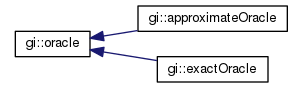
\includegraphics[ width=0.7\textwidth]{EreditaOracolo}
	\caption[Ereditarietà Oracolo]{Ereditarietà Oracolo}
   \label{fig:eor}
\end{figure}

L'algoritmo \ac{ObP} invece di possedere (composizione) un \ac{DFA} target ha un oggetto della classe base astratta Oracolo. Quando si invoca il costruttore dell' \ac{ObP}  si deve passare anche l'indirizzo di un oggetto della classe Oracolo. Tramite il tipo di oggetto Oracolo(si ha un handle della classe base Oracolo che punta allo specifico oggetto della classe derivata passato) passato  viene determinato in maniera trasparente con il polimorfismo se si desidera utilizzare l'\ac{ObP} piuttosto che l'\ac{ObPA}. Le chiamate alle funzioni effettuate sull'oggetto Oracolo all'interno di \ac{ObP} hanno la stessa \textit{signature} , cioè le \ac{MQ} e le \ac{EQ} , ma il tipo dell'oggetto Oracolo passato determina automaticamente di quale classe derivata invocare le funzioni (che avranno diverse implementazioni a secondo se appartengono alla classe exactOracle o a quella approximateOracle).  In questo modo la classe dell'algoritmo \ac{ObP} ha subito pochissime modifiche  e il lavoro d'implementazione di questa tesi si è focalizzato sulla classe approximateOracle. Infine all'interno della classe observation\_pack , per impedire al \textit{client} di vedere le strutture dati e le modifiche effettuate su di esse  e in ultimo il modo in cui funziona l'algoritmo, è necessario effettuare una copia interna dell'Oracolo passato dal \textit{client} ma non conoscendo a priori di quale tipo, e quindi di quale classe, è l'Oracolo vi è stata la difficoltà su come invocare il costruttore di copia. A tal fine si è usata la tecnica del \textit{clone idiom} .Quando si ha un riferimento polimorfico cioè un 
  puntatore alla classe base che punta a un oggetto della classe derivata all'occorrenza può sorgere il problema di determinare qual è il tipo della classe derivata . Allora nella classe base si dichiara un metodo virtuale puro che tutte le classi derivate devono quindi implementare. Quest'implementazione consiste nella creazione dinamica  di un nuovo oggetto della classe derivata chiamando il costruttore di copia della classe derivata sull'oggetto corrente (tramite new classeDerivata(*this)). Questo nuovo oggetto creato verrà tornato al chiamante. Si noti che il costruttore di copia della classe derivata deve provvedere a chiamare il costruttore di copia della classe base e che in questi costruttori deve avvenire una deep copy di tutti i membri dinamici.   In figura \ref{fig:cba} l'interfaccia della classe base astratta.
  
 \begin{figure}[htp]
	\centering
	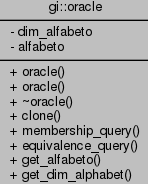
\includegraphics[ width=0.3\textwidth]{Oracolo}
	\caption[Interfaccia classe base Oracolo]{Interfaccia classe base Oracolo}
   \label{fig:cba}
\end{figure}    